
\section{Anforderungen} % (TODO!): Henning schreibt das.

% Hinweistext Skript zum Modul: Welche Techniken/ Technologien sollen eingesetzt werden, um die Aufgabe zu lösen/ realisieren? Warum sollen gerade diese eingesetzt werden? Gibt es besondere Anforderungen? (technisch, Benutzer, sonstige)

% \footnote{Technologie-Stack nach \url{https://mixpanel.com/de/blog/was-ist-ein-technologie-stack/}: \enquote{Ein Technologie-Stack, auch Lösungs-Stack, Technologie-Infrastruktur oder Datenökosystem genannt, ist eine Liste aller Technologiedienste, die zum Aufbau und Ausführen einer einzelnen Anwendung verwendet werden}}

Die Anforderungen an das Projekt wurden aus verschiedenen Quellen definiert. Hier zum einen allein schon durch das Modulthema \enquote{\textbf{Web Technologie}} sowie weiter im Allgemeinen sowie im Speziellen durch den \textbf{Dozenten} als auch abschließend auch durch uns als \textbf{Projektteam} selbst. 

Das Modulthema gibt hierbei das grundsätzliche Umfeld vor und bestimmt damit auch wesentlich alle weiteren Details folgender Anforderungen. Der Dozent gab hier allgemeine Anforderungen an alle Teilnehmende des Moduls, und definierte weiter auch spezielle Anforderungen an die Durchführung unseres Projektes. Eine dritte Menge von Anforderungen entstand aus unseren eigenen Projektbesprechungen und -abstimmungen.  

All diese Anforderungen wurden gebündelt in der Projektbesprechung vom 27.11.2021 erfasst, von uns bewertet und zusammen in eine Projektskizze (siehe folgend Bilder \ref{fig:2021-11-27-projektskizze-1} und \ref{fig:2021-11-27-projektskizze-2}) transportiert. Mit den darin erfassten Inhalten unter den Punkten \textbf{Zielsetzung}, \textbf{Aufgaben und Ergebnisse} sowie \textbf{Randbedingungen} wurden alle gestellten Anforderungen systematisch erfasst und damit sichergestellt, dass diese im Projektverlauf auch entsprechend Beachtung finden und erledigt werden. 


\begin{figure}[H]N
    \centering
    \caption{Projektsizee aus Projektbesprechung vom 27.11.2021, Teil 1}
    \label{fig:2021-11-27-projektskizze-1}
    \fbox{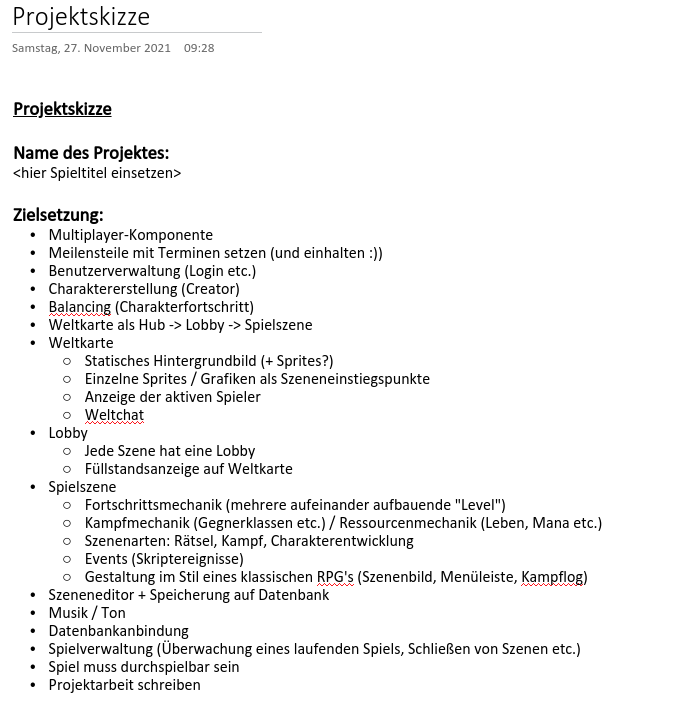
\includegraphics[width=0.7\textwidth]{2021-11-27-projektskizze-1}}
\end{figure}


\begin{figure}[H]
    \centering
    \caption{Projektsizee aus Projektbesprechung vom 27.11.2021, Teil 2}
    \label{fig:2021-11-27-projektskizze-2}
    \fbox{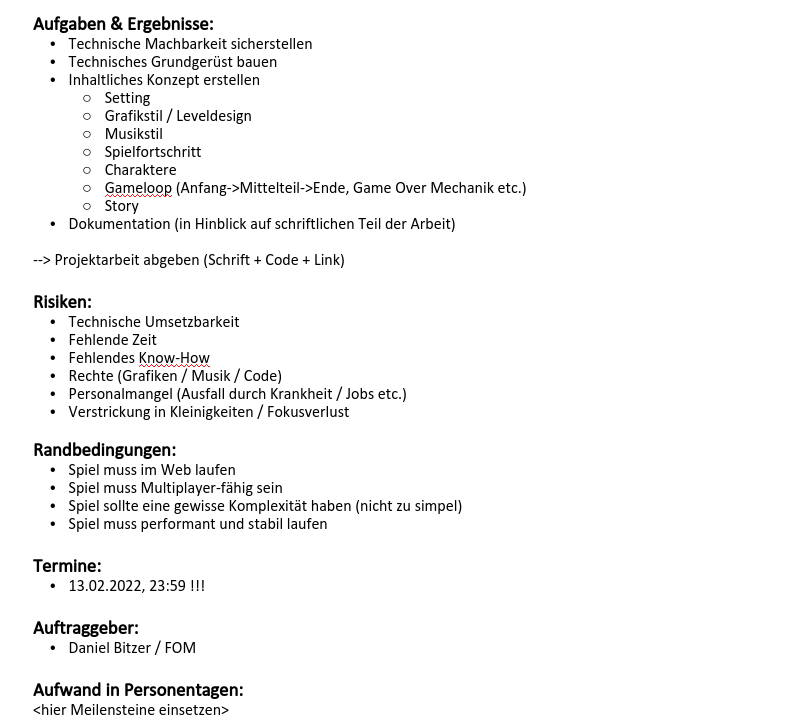
\includegraphics[width=0.7\textwidth]{2021-11-27-projektskizze-2}}
\end{figure}

Die wensentlichen Anforderungen, deren Erfüllbarkeit vorallem auch an die gewählten Technologien gebunden sind, wurden wie folgt besimmt: Das Spiel muss... \begin{itemize}
    \item ...im Web laufen.
    \item ...multiplayerfähig sein.
    \item ...eine gewisse Komplexität (Charkterentwicklung, Klassen) haben.
    \item ...performant und stabil laufen.
\end{itemize}

%TO-DO?: Müssen hier vielleicht auch Techniken/Technologien für Frontend- / Grafik- und Game-Design rein? Zumindest verwendete Programme/Modelle/Best Practices etc. sollten denke ich erwähnt werden
% Was ist mit Github? 

Die Anforderungen \enquote{im Web laufen} sowie \enquote{performant und stabil} sind bei korrekter Konfiguration, entsprechender Hardware und Wartung durch nahezu jeden \ac{Stack} zu erfüllen. 

Da das gesamte Projektteam unerfahren mit der Umsetzung von Webprojekten war und die ersten, in den Vorlesungen zum Modul gesammelten Erfahrungen, mit der dort Vorgestellten Lösung \textbf{Django} durchweg positiv waren, wurde dem eine deutliche Präferenz zugeschrieben. Die zuerst genannten Anforderungen, dürfen bei Django auch als erfüllt betrachtet werden. Django ist weit verbreitet und wird produktiv im gewerblichen Einsatz erfolgreich betrieben. 

Die nächste Anforderung \enquote{multiplayerfähig}, stellte bereits höhere Ansprüche and die eingesetzte Technologie. Zuerst war hier zu klären bzw. zu definieren, wie genau der Ablauf des Spiels sein soll. Auch musste festgelegt werden welche Arten von Interaktion zwischen dem Spiel und den Spielern und auch unter den Spielern selbst gewünscht sind. 

Wir haben hier in Projektbesprechungen schnell erkannt, dass das Spiel mit allen möglichen Interaktionen, jeweils einzeln genau definiert werden müssen. Nur so lassen sich konkrete Anforderungen formulieren und die spätere Programmierung erledigen. 

Bei dieser Definition wurde weiter deutlich, dass es (bedingt duch die geforderte Multiplayerfähigkeit) nicht nur einen bedeutenden Aufwand zu Entwurf und Programmierung bezüglich der Spiellogik selbst, sondern auch bezüglich des \textbf{\gls{Matchmaking}} geben wird. 

Das \gls{Matchmaking} sollte hier nicht automatisch erfolgen, sondern bewusst durch die Spieler. Ein gewisser Austausch ist dafür unabdingbar: Es wurde eine Chat-Funktion bennötigt. Über eine Recherche dazu, wurden wir auf das \textbf{Websocket-Protokoll} aufmerksam. Gemäß der Beschreibung nach \citeauthor{heise-django-2011} (\citeyear{heise-django-2011}) sollten unsere Anforderungen umfassend erfüllt werden. Das Websocket-Protkoll ist -ähnlich einer TCP-Verbindung- eine bestehen bleibende Verbindung, die es auch erlaubt Events von Serverseite aus, an den Client (ohne dessen gesonderte Anforderung), zu übertragen. 

An vielen Stellen im Projekt, würde dies eine Anforderung sein, die mit den Websockets damit erfüllt werden konnten. 

Alternative Frameworks (Backend, als auch Frontend) waren uns zwar teilweise vom Namen bekannt, wurden aber weiter nicht genauer in Betracht gezogen. Auch damit grundsätzliche Erfahungen im Umgang mit HTML, CSS und JavaScript im Rahmen des Projkets durch das Team gesammelt werden können. Die Abkürzung über ein Framework wurde daher hier auch bewusst nicht gewählt. 

